\documentclass[edipack2.tex]{subfiles}
\begin{document}

\section{Examples}\label{SecExamples}
In this section we illustrate the functioning of the \NAME
library and their interfaces as solver for DMFT through specific examples, including
discussion of relevant code snippets. 


\subsection{Bethe lattice DMFT}\label{SecExamplesBetheDMFT}
The test bed for any DMFT application is conventionally considered 
the description of the Mott or metal-to-insulator transition (MIT) 
in a Bethe lattice, i.e., a Cayley tree with coordination number 
$z\to\infty$~\cite{Georges1996}.
Here, we present a guided implementation of the DMFT 
solution for the Bethe lattice at $T=0$ using \NAME as impurity
solver.
The model under consideration is the Fermi-Hubbard Hamiltonian:
$$
H = -t \sum_{\langle ij\rangle,\s} c^\dagger_{i\s} c_{j\s} + 
    U \sum_i n_{i\up}n_{i\dw}
    $$
    
where $c^\dagger_{i\s}$ ($c_{i\s}$) are the creation (annihilation) 
operators for an electron at site $i$ with spin $\s$, and 
$n_{i\s} = c^\dagger_{i\s} c_{i\s}$ is the corresponding occupation 
operator. The first sum runs over nearest-neighbor pairs 
$\langle ij \rangle$.

The system is defined on a Bethe lattice with density of states
$\rho(\e)=\frac{1}{2D}\sqrt{D^2-\e^2}$,
where $D=2t$ is the half-bandwidth.
In DMFT this lattice model is mapped onto a quantum impurity problem with 
an effective electronic bath that must be determined
self-consistently.

Below, we present the key components of a basic DMFT implementation 
using \NAME for the Bethe lattice, employing either the Fortran or 
C++ APIs. Fully operational versions of the two codes can be found 
in the {\tt examples} directory of the \NAME source code. Both 
samples share a similar initial structure, including memory 
allocation, Bethe lattice creation, and solver initialization.

\setbox0=\hbox{%
  \begin{minipage}{0.465\linewidth}
    \center{\bf Fortran}
\begin{lstlisting}[style=fstyle,frame=none,numbers=none,basicstyle={\scriptsize\ttfamily}]
program ed_hm_bethe
   USE EDIPACK2
   USE SCIFOR
   implicit none
   integer                :: Le=1000
   real(8)                :: wmixing=0.5d0
   real(8)                :: D=1d0
   integer                :: Nb
   real(8),allocatable    :: Bath(:)
   complex(8),allocatable :: Hloc(:,:,:,:)
   real(8),allocatable    :: Ebands(:),Dbands(:)
   complex(8),allocatable :: Smats(:,:,:,:,:)
   complex(8),allocatable :: Delta(:,:,:,:,:)
   ...  
   !Read variables
   call ed_read_input('inputED.conf')
   !Solver-specific arays
   allocate(Smats(Nspin,Nspin,Norb,Norb,Lmats))
   allocate(Delta(Nspin,Nspin,Norb,Norb,Lmats))
   allocate(Hloc(Nspin,Nspin,Norb,Norb));Hloc=0d0
   ...
   !Initialize Bethe arrays
   allocate(Ebands(Le),Dbands(Le))
   Ebands = linspace(-D,D,Le,mesh=de)
   Dbands = dens_bethe(Ebands,Wband)*de
   !Set local H
   call ed_set_hloc(Hloc)
\end{lstlisting}
\end{minipage}
}
\savestack{\listingA}{\box0}

\setbox0=\hbox{%
  \begin{minipage}{0.505\linewidth}
    \center{\bf C++}
\begin{lstlisting}[style=cstyle,frame=none,numbers=none,basicstyle={\scriptsize\ttfamily}]
#include <edipack2_cbinding.h>
using namespace std;
...
//Main variables
int Le = 1000;
int iloop = 0;
double wmixing = 0.5;
double D = 1.0;
//Read  variables    
char input[] = "inputED.conf"; 
read_input(input);      
//Dimensions
int64_t d[4] = {Nspin,Nspin,Norb,Norb};
int total_size = d[0] * d[1] * d[2] * d[3];
int total_size_n5 = total_size * Lmats;    
// Solver-specific arrays
vector<complex<double>> Hloc(total_size);
vector<complex<double>> Smats(total_size_n5);
vector<complex<double>> Delta(total_size_n5);
...
// Initialize Bethe arrays
vector<double> Ebands, Dbands;
Ebands = linspace(-D,D,Le);
Dbands = dens_bethe(Ebands,Wband,de);
//set local H
ed_set_Hloc_single_N4(Hloc.data(), d);
\end{lstlisting}
\end{minipage}
}
\savestack{\listingB}{\box0}

\begin{tabular}{c|c}\label{list2}
  \stackinset{l}{}{t}{}{}{\listingA} & \stackinset{l}{}{t}{}{}{\listingB} 
\end{tabular}

The bath is described by the (unknown) function $\GG^{-1}_0$, known as 
the Weiss field ({\tt Weiss}). In the ED approach implemented in \NAME, 
the bath is approximated using a finite number of discrete energy levels. 
The function $\GG^{-1}_0$ is then used to determine the bath parameters 
$\vec{x} = \{V, h\}$ through the optimization method outlined in 
\secu{sSecFit}.

The starting point for any calculation is a reasonable initial guess 
for the Weiss field, or equivalently, the bath parameters. In \NAME, 
this is accomplished using the function {\tt
  ed\_init\_solver} (Fortran API) or {\tt init\_solver\_site} (C++ API).

\setbox0=\hbox{%
  \begin{minipage}{0.465\linewidth}
    \center
    \begin{lstlisting}[style=fstyle,frame=none,numbers=none,basicstyle={\scriptsize\ttfamily}]
   !Initialize solver
   Nb=ed_get_bath_dimension()
   allocate(bath(Nb))
   call ed_init_solver(bath)
\end{lstlisting}
\end{minipage}
}
\savestack{\listingA}{\box0}

\setbox0=\hbox{%
  \begin{minipage}{0.505\linewidth}
    \center
\begin{lstlisting}[style=cstyle,frame=none,numbers=none,basicstyle={\scriptsize\ttfamily}]
// Initialize solver
int Nb;
vector<double> Bath(Nb);
Nb = get_bath_dimension();
int64_t bath_dim[1] = {Nb};
init_solver_site(Bath.data(), bath_dim);
\end{lstlisting}
\end{minipage}
}
\savestack{\listingB}{\box0}

\begin{tabular}{c|c}\label{list2}
  \stackinset{l}{}{t}{}{}{\listingA} & \stackinset{l}{}{t}{}{}{\listingB} 
\end{tabular}


The iterative algorithm to solve the DMFT problem is based on
a reverse communication strategy and proceeds as follows:
\begin{itemize}
  
\item[{\tiny $\blacksquare$}] Call the exact diagonalization {\bf impurity solver}
  whose only input is the set of parameters $\vec{x}$ contained in a
  rank-1 array. All  \NAME options are controlled through input file
  specifications.
  
\item[{\tiny $\blacksquare$}] Retrieve the self-energy functions $\Sigma_{\a\b\s\s'}(i\omega)$ on the
  Matsubara axis using dedicated function provided by \NAME API.
  
\item[{\tiny $\blacktriangleright$}] Evaluate the local interacting Green's function
  $G_\mathrm{loc}(i\omega) = \int_{-D}^D \frac{\rho(\e)}{\zeta -\e}d\e$ with
  $\zeta=i\omega+\mu-h^0-\Sigma(i\omega)$.
  
\item[{\tiny $\blacktriangleright$}] Update the Weiss field via the {\bf self-consistency}
  relation: $\GG^{-1}_0(i\omega) = G_\mathrm{loc}(i\omega) +
    \Sigma(i\omega)$. For the Bethe lattice, this simplifies to
    $\Delta = \tfrac{D}{4}G_\mathrm{loc}$.
    
  \item[{\tiny $\triangleright$}] Optimize the bath parameters $\vec{x}$ against the updated
    Weiss field,  potentially using the conjugate gradient procedures 
supplied by \NAME. Then, restart at step 1.
\end{itemize}

The first two steps, marked by the ${\tiny \blacksquare}$ symbol, 
are handled directly by \NAME routines. In the subsequent steps, 
indicated by the ${\tiny \blacktriangleright}$ symbol, control returns 
to the user, who must implement the algebraic updates required to 
close the self-consistency loop and optimize the bath.
Given the 
critical importance of this optimization, \NAME provides access to 
well-tested functions, ensuring stability and reproducibility of 
results. Alternative optimization methods can also be employed as 
needed. 
An example of implementation is provided in the following listings.


\setbox0=\hbox{%
  \begin{minipage}{0.45\linewidth}
    \center
    \begin{lstlisting}[style=fstyle,frame=none,numbers=none,basicstyle={\scriptsize\ttfamily}]
!DMFT loop
do while(.not.converged.AND.iloop<nloop)
    iloop=iloop+1     
    ! Call ED Solver
    call ed_solve(bath)     
    ! Retrieve Self-energy on Matsubara axis
    call ed_get_sigma(Smats,'m')
    ! Build local Green's function
    wfreq = pi/beta*(2*arange(1,Lmats)-1)
    do i=1,Lmats
       zeta= xi*wfreq(i)+xmu - Smats(1,1,1,1,i)
       Gmats(1,1,1,1,i)=sum(DOS/(zeta-Ene))*de  
    enddo
    ! Self-consistency
    Delta = D/4d0*Gmats
    ! Fitting -> new bath
    call ed_chi2_fitgf(Weiss,bath,ispin=1)     
    ! Check convergence
    converged=check_convergence(Delta,&
          dmft_error,Nsuccess,Nloop)
enddo
\end{lstlisting}
\end{minipage}
}
\savestack{\listingA}{\box0}

\setbox0=\hbox{%
  \begin{minipage}{0.52\linewidth}
    \center
\begin{lstlisting}[style=cstyle,frame=none,numbers=none,basicstyle={\scriptsize\ttfamily}]
  // DMFT loop
  while (iloop < Nloop && !converged) {
    //  Call ED Solver
    solve_site(Bath.data(),bath_dim,1,1);      
    // Retrieve  Self-energy on Matsubara axis
    get_sigma_site_n5(Smats.data(),//
        0,0,wm.data(),Lmats,0);
    //  Build a local Green's function:
    for (int i=0;i<Lmats;++i) {
      zeta= wm[i] + xmu - Smats[i];
      Gmats[i] = complex<double>(0.0,0.0);
      for (int j=0; j< Le; j++) {
        Gmats[i]+=Dbands[j]/(zeta-Ebands[j]);
      }
    }
    // Self-consistency
    for (int i = 0; i < Lmats; ++i) {
      Delta[i] = 0.25 * D * Gmats[i];
    }
    // Fit -> new bath
    chi2_fitgf_single_normal_n5(Delta.data(),//
        delta_dim,Bath.data(),bath_dim,1,0,1);
    // Check convergence
    converged = check_convergence(Delta,//
        dmft_error, Nsuccess, Nloop, comm);  
  }
\end{lstlisting}
\end{minipage}
}
\savestack{\listingB}{\box0}

\begin{tabular}{c|c}\label{list2}
  \stackinset{l}{}{t}{}{}{\listingA} & \stackinset{l}{}{t}{}{}{\listingB} 
\end{tabular}




\paragraph{Results}
In the following, we present results for the interaction-driven Mott 
transition in the Bethe lattice, which captures the gradual 
transformation of a partially-filled metallic state into a correlated 
insulator.
To illustrate this, we report in panel (A) the evolution of the spectral 
function $-{\rm Im}G_\mathrm{loc}(\omega)/\pi$ as a function of the 
interaction strength $U$. Despite the inherently {\it spiky} nature 
of the spectrum, resulting from the finite number of poles in the 
discretized effective bath, the characteristic features of the Mott 
transition are clearly visible. At low energies, a renormalized 
quasi-particle peak develops at the Fermi level ($\omega = 0$). 
Simultaneously, the system exhibits the formation of incoherent 
high-energy features, which eventually evolve into well-defined 
Hubbard bands in the Mott insulating phase for $U > U_\mathrm{c}$, 
with $U_\mathrm{c} \simeq 2.8D$.

\begin{figure}[t!]
  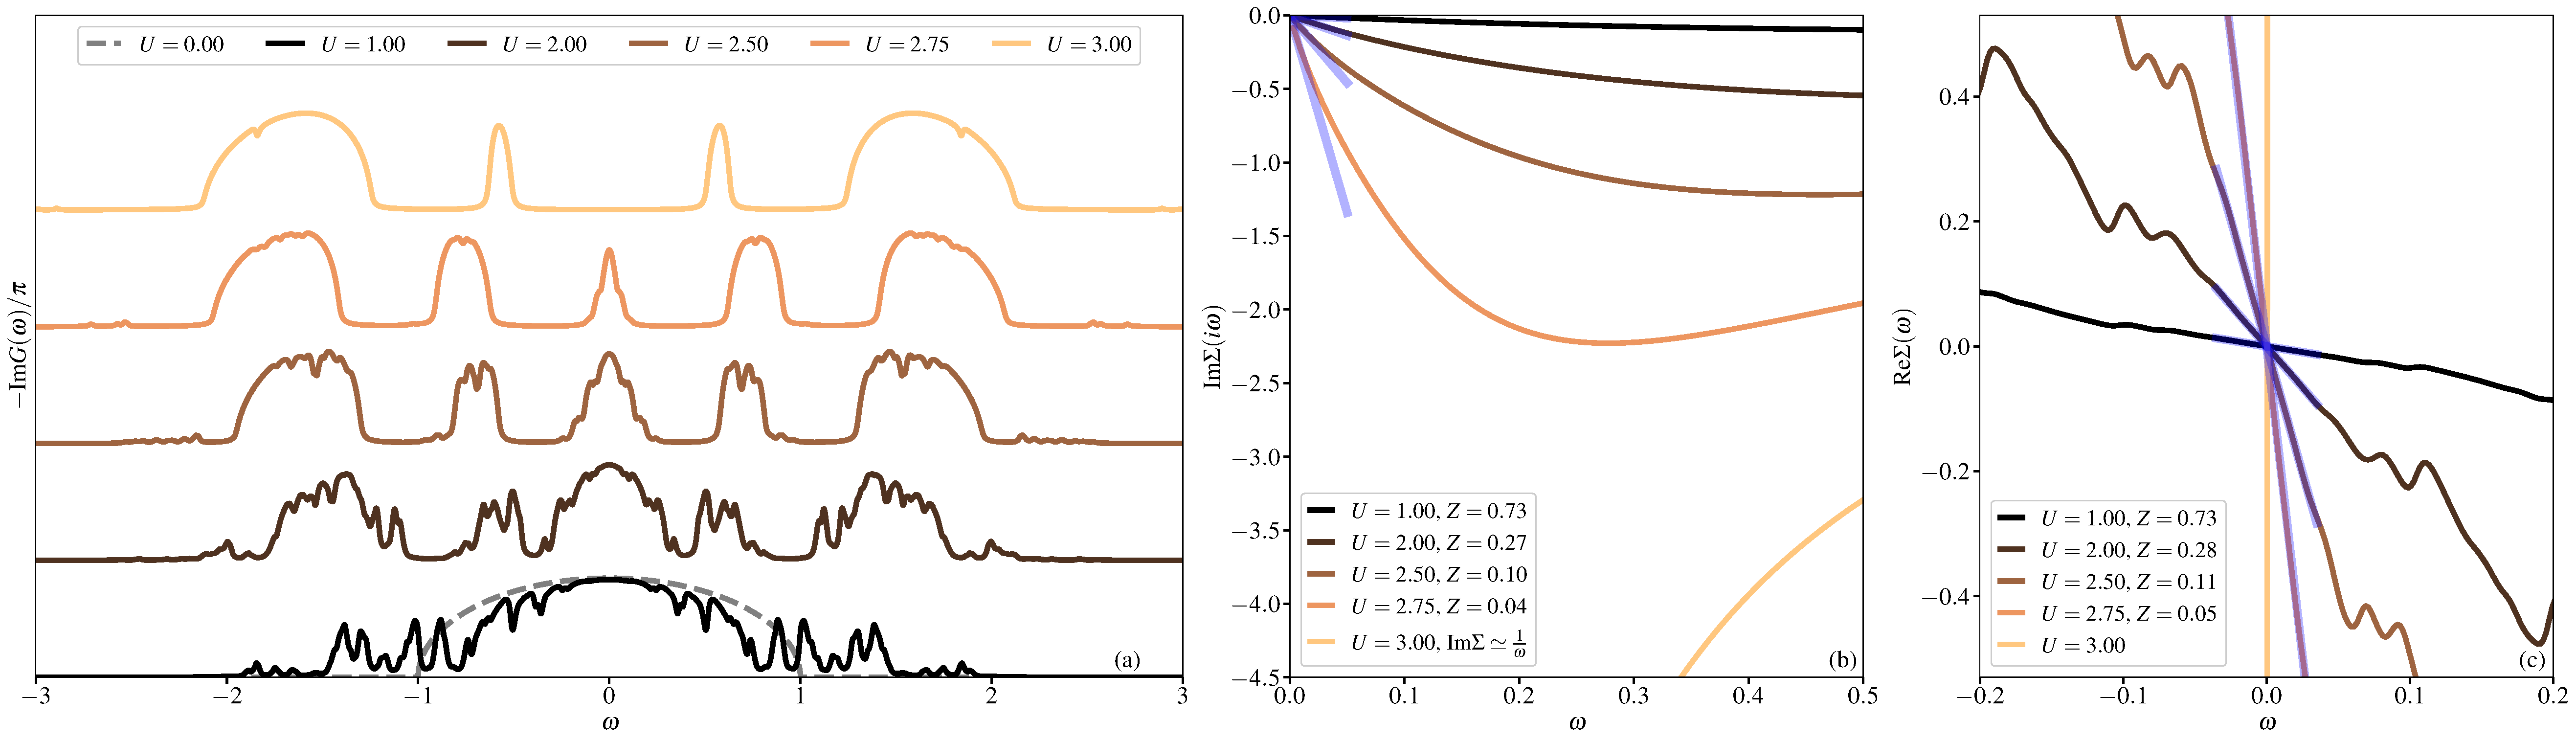
\includegraphics[width=\linewidth]{figures/figBethe.pdf}
    \caption{\label{figEx1}%
      \textbf{The Metal-Insulator Mott transition.}
      (a) Evolution of the spectral function $-\Im{G}(\omega)/\pi$ as
      a function of increasing interaction $U$. The critical
      interaction $U_\mathrm{c}\simeq 2.8D$ separates the correlated metal $U<U_\mathrm{c}$ from
      the Mott insulator $U>U_\mathrm{c}$.
      (b)-(c) The corresponding evolution of the Matsubara self-energy
      $\Im\Sigma(i\omega)$ (b) and
      real-axis one $\Re\Sigma(\omega)$ across the Mott
      transition. For a particle-hole symmetric case both allow to
      estimate the renormalization constant $Z$ (see main text), using
      linear order expansion in frequency (blue solid lines). The
      values of $Z$ are reported in the legend.
      The Mott insulating solution is associated to a singularity at
      $\omega=0$ of $\Im\Sigma$. 
        }
\end{figure}

The formation of a spectral gap separating the Hubbard bands in the 
Mott insulating phase is associated with the divergence of the 
imaginary part of the self-energy at the Fermi level. This divergence 
reflects the complete localization of the electrons, effectively 
suppressing coherent quasi-particle excitations. Specifically, 
causality dictates that the real part of the self-energy must also 
grow significantly near the singularity, making it impossible to 
satisfy the quasi-particle pole equation
$$
\omega+\mu-h^0-\e-\Re{\Sigma}(\omega)=0,
$$
which governs the formation of coherent excitations near the Fermi 
level.

Panels (B) and (C) illustrate this phenomenon by showing the evolution 
of the self-energy $\Sigma$. In panel (B), we present the Matsubara 
self-energy ${\rm Im}\Sigma(i\omega)$ in the low-energy regime. As the 
interaction strength $U$ increases, this function progressively 
grows, eventually diverging as the critical interaction threshold 
$U > U_\mathrm{c}$ is crossed.
This divergence along the Matsubara axis is directly linked to the
particle-hole symmetry of the Bethe lattice, which pins the  ${\rm
  Im}\Sigma$ singularity at $\omega = 0$.

Panel (C) complements this picture by displaying the real part 
$\Re{\Sigma}(\omega)$ in the same low-energy regime. Here, increasing 
$U$ leads to a rapid rise of this component, culminating in a 
discontinuous behavior as the critical point is approached. This 
discontinuity directly reflects the divergence in the imaginary part
on the real-axis,  confirming the transition to the Mott insulating state.


A quantitative measure of this transition is provided by the 
quasi-particle renormalization factor $Z$, which can be used to capture the degree 
of electron delocalization. This parameter ranges from 1 for a 
non-interacting metal to 0 for a fully localized Mott insulator. It is 
defined through the low-energy expansion of the self-energy as
$$
Z=(1-\tfrac{\partial\Re\Sigma}{\partial\omega}_{|_{\omega\rightarrow
    0}})^{-1}.
$$
which can also be estimated from the linear behavior of ${\rm Im}\Sigma(i\omega)$ for 
$\omega\to0$ in the metallic regime using the relation:
$$
   \frac{\Im\Sigma(i\omega_n)}{\omega_n}_{|_{\omega_n\rightarrow 0}}=
   \frac{1}{\pi}\int_{\mathbb R}d\epsilon \frac{\Re\Sigma(\epsilon)}{\epsilon^2}=
   \frac{\partial\Re\Sigma}{\partial\omega}_{|_{\omega\rightarrow 0}}.
$$

The linear fits highlighted in panels (B) and (C), along with the 
corresponding $Z$ values provided in the legends, clearly indicate that 
the slope of the self-energy at low energy increases with $U$ on both 
the Matsubara and real axes. At the transition point, this slope 
diverges, reflecting the onset of complete electron localization as 
$Z \to 0$, consistent with the divergence 
${\rm Im}\Sigma(\omega) \rightarrow -\infty$.






















\subsection{Attractive Hubbard model}\label{SecExamplesAHM}
The second example we present concerns the DMFT description of the 
attractive Hubbard model on a two-dimensional square lattice. This 
example has a twofold aim: (i) to demonstrate the support of \NAME 
for ($s$-wave) superconductivity, and (ii) to illustrate the use of 
the library's Python API through a concrete working example. The 
model Hamiltonian is given by:
$$
H = \sum_{\ka,\s} \epsilon(\ka) c^\dagger_{\ka\s} c_{\ka\s} 
    - U \sum_i n_{i\up} n_{i\dw},
$$
where $U > 0$, $c^\dagger_{\ka\s} = \tfrac{1}{\sqrt{N}} 
\sum_i e^{-i\ka \cdot R_i} c^\dagger_{i\s}$, and $c^\dagger_{i\s}$ 
is the creation operator for an electron at site $i$ with spin $\s$. 
The occupation operator is $n_{i\s} = c^\dagger_{i\s} c_{i\s}$, and 
the energy dispersion relation is $\e(\ka)=-2t[\cos{(k_x a)}+
\cos{(k_y a)}]$, where we set the lattice spacing 
$a=1$  and the choose the energy unit such as $4t=D=1$ for convenience.

The DMFT workflow for this case is largely similar to the previous 
example, but it now operates in the Nambu basis defined by the spinor
$$
\psi_i=\begin{bmatrix} c_{i\up} \\ c^\dagger_{i\dw} \end{bmatrix}. 
$$
In this basis, the Green's function takes the matrix form:
\begin{equation}
  {\mathbf G} =
  \begin{pmatrix}
    \hat{G}_{\uparrow\uparrow} & \hat{F}_{\uparrow\downarrow}\\
    \hat{\bar{F}}_{\downarrow\uparrow}  &    \hat{\bar{G}}_{\downarrow\downarrow} \\
  \end{pmatrix}
\end{equation}
where the symbol $\hat{A}$ indicates the potential multi-orbital 
nature of the system, which reduces to a scalar in the present 
single-orbital case. The components in the second row, denoted 
by $\hat{\bar{A}}$, are connected to the first row by particle-hole 
and time-reversal symmetries. The specific relations depend on the 
symmetry of the order parameter (here, $s$-wave) and whether the 
functions are defined on the Matsubara or real-frequency axis:
\begin{equation}
\begin{array}{cc}
  \hat{\bar{G}}(i\omega) = -\hat{G}^*(i\omega)\;; &  \hat{\bar{F}}(i\omega) = \hat{F}(i\omega)\\
  \hat{\bar{G}}(\omega)  = -\hat{G}^*(-\omega) \;; & \hat{\bar{F}}(\omega) = \hat{F}^*(i\omega)\\
\end{array}
\end{equation}  

The code implementation closely follows the structure of the previous 
example, with some notable adjustments related to the Nambu basis. 
Specifically, the above symmetries allow one to compute only the 
independent components from the first row, significantly reducing 
the computational effort. The initial part of the code handles the 
lattice structure and solver initialization, as described below.

\begin{lstlisting}[style=mypython,numbers=none,basicstyle={\scriptsize\ttfamily}]
import numpy as np
from edipy2 import global_env as ed
import mpi4py
from mpi4py import MPI
import os,sys
from aux_funx import * #include function to build $G_\mathrm{loc}$ 
comm = MPI.COMM_WORLD
rank = comm.Get_rank()
master = (rank==0)
#Functions
def generate_kgrid(Nk):
    b1=2*np.pi*np.array([1.0,0.0])
    b2=2*np.pi*np.array([0.0,1.0])
    n1, n2 = np.meshgrid(np.arange(Nk), np.arange(Nk))
    n1=n1/Nk;n2=n2/Nk
    gridout = np.stack([n1.ravel(), n2.ravel()], axis=-1)
    return np.dot(gridout,[b1,b2])
def h_square2d(k,t):
  return -2*t*(np.cos(k[...,0,np.newaxis,np.newaxis])+np.cos(k[...,1,np.newaxis,np.newaxis]))*np.eye(ed.Norb)
    
#Read input
ed.read_input("inputAHM.conf")

#Generate Hk and  set Hloc
kgrid = generate_kgrid(Nk)
Hk   = h_square2d(kgrid,t_hop)
HkNambu   = np.array([h_square2d(kgrid,t_hop),-np.conj(h_square2d(-kgrid,t_hop))])
Hloc = np.sum(Hk,axis=0)/Nk**2
ed.set_hloc(Hloc.astype(complex))

#Setup ED Solver
Nb=ed.get_bath_dimension()
bath = ed.init_solver()
\end{lstlisting}



The iterative scheme for the solution of DMFT closely follows the
sequence already discussed in \secu{SecExamplesBetheDMFT}:   
\begin{itemize}
\item Call the exact diagonalization {\bf impurity solver} {\tt
    ed.solve} providing the set of bath parameters $\vec{x}=\{V,h\}$  as input. 

\item Use the dedicated
  input/output \NAME procedures to retrieve the self-energy functions  
  $\hat{\Sigma}(i\omega)$ and $\hat{S}(i\omega)$ on the 
  Matsubara axis.
  
\item
  Evaluate the interacting local Green's functions $\hat{G}_\mathrm{loc}$ and
  $\hat{F}_\mathrm{loc}$:
  \begin{equation}
  {\mathbf G}_\mathrm{loc}(i\omega) =
  \int_\RRR d\e \rho(\e)
  \begin{pmatrix}
    (i\omega +\mu)\hat{\11} - \hat{h}^0 - \hat{\Sigma}(i\omega) -\e & -\hat{S}(i\omega) \\
    -\hat{S}(i\omega) & (i\omega +\mu)\hat{\11} + \hat{h}^0 +
    \hat{\Sigma}^*(i\omega) +\e\\
  \end{pmatrix}^{-1}
\end{equation}

\item Update the Weiss fields components, respectively 
  $\GG_0^{-1}$ and $\FF_0^{-1}$, through the {\bf self-con\-sis\-ten\-cy}
  relation: $\mathbfcal{G}^{-1}_0(i\omega) = {\mathbf G}_\mathrm{loc}(i\omega) +
  {\mathbf \Sigma}(i\omega)$ in Nambu space.
  
\item Optimize the bath parameters $\vec{x}$ to best describe the updated
    Weiss fields, potentially using \NAME provided conjugate gradient  fit
    procedures.
  \end{itemize}
%
The corresponding implementation in Python reads:
\begin{lstlisting}[style=mypython,numbers=none,basicstyle={\scriptsize\ttfamily}]
#DMFT CYCLE
converged=False;iloop=0
while (not converged and iloop<ed.Nloop ):
    iloop=iloop+1
    #Solve impurity problem
    ed.solve(bath)    
    #Self-consistency with aux_funx procedures:
    Smats = np.array([ed.get_sigma(axis="m",typ="n"),ed.get_sigma(axis="m",typ="a")])    
    Gmats = get_gloc(wm*1j       ,ed.xmu,HkNambu,Smats,axis="m") 
    Weiss = dmft_weiss_field(Gmats,Smats)                            
    #Fit
    bath = ed.chi2_fitgf(Weiss[0],Weiss[1],bath)
    #Error check
    err,converged=ed.check_convergence(Weiss,ed.dmft_error)
ed.finalize_solver()
\end{lstlisting}


\begin{figure}[t!]
  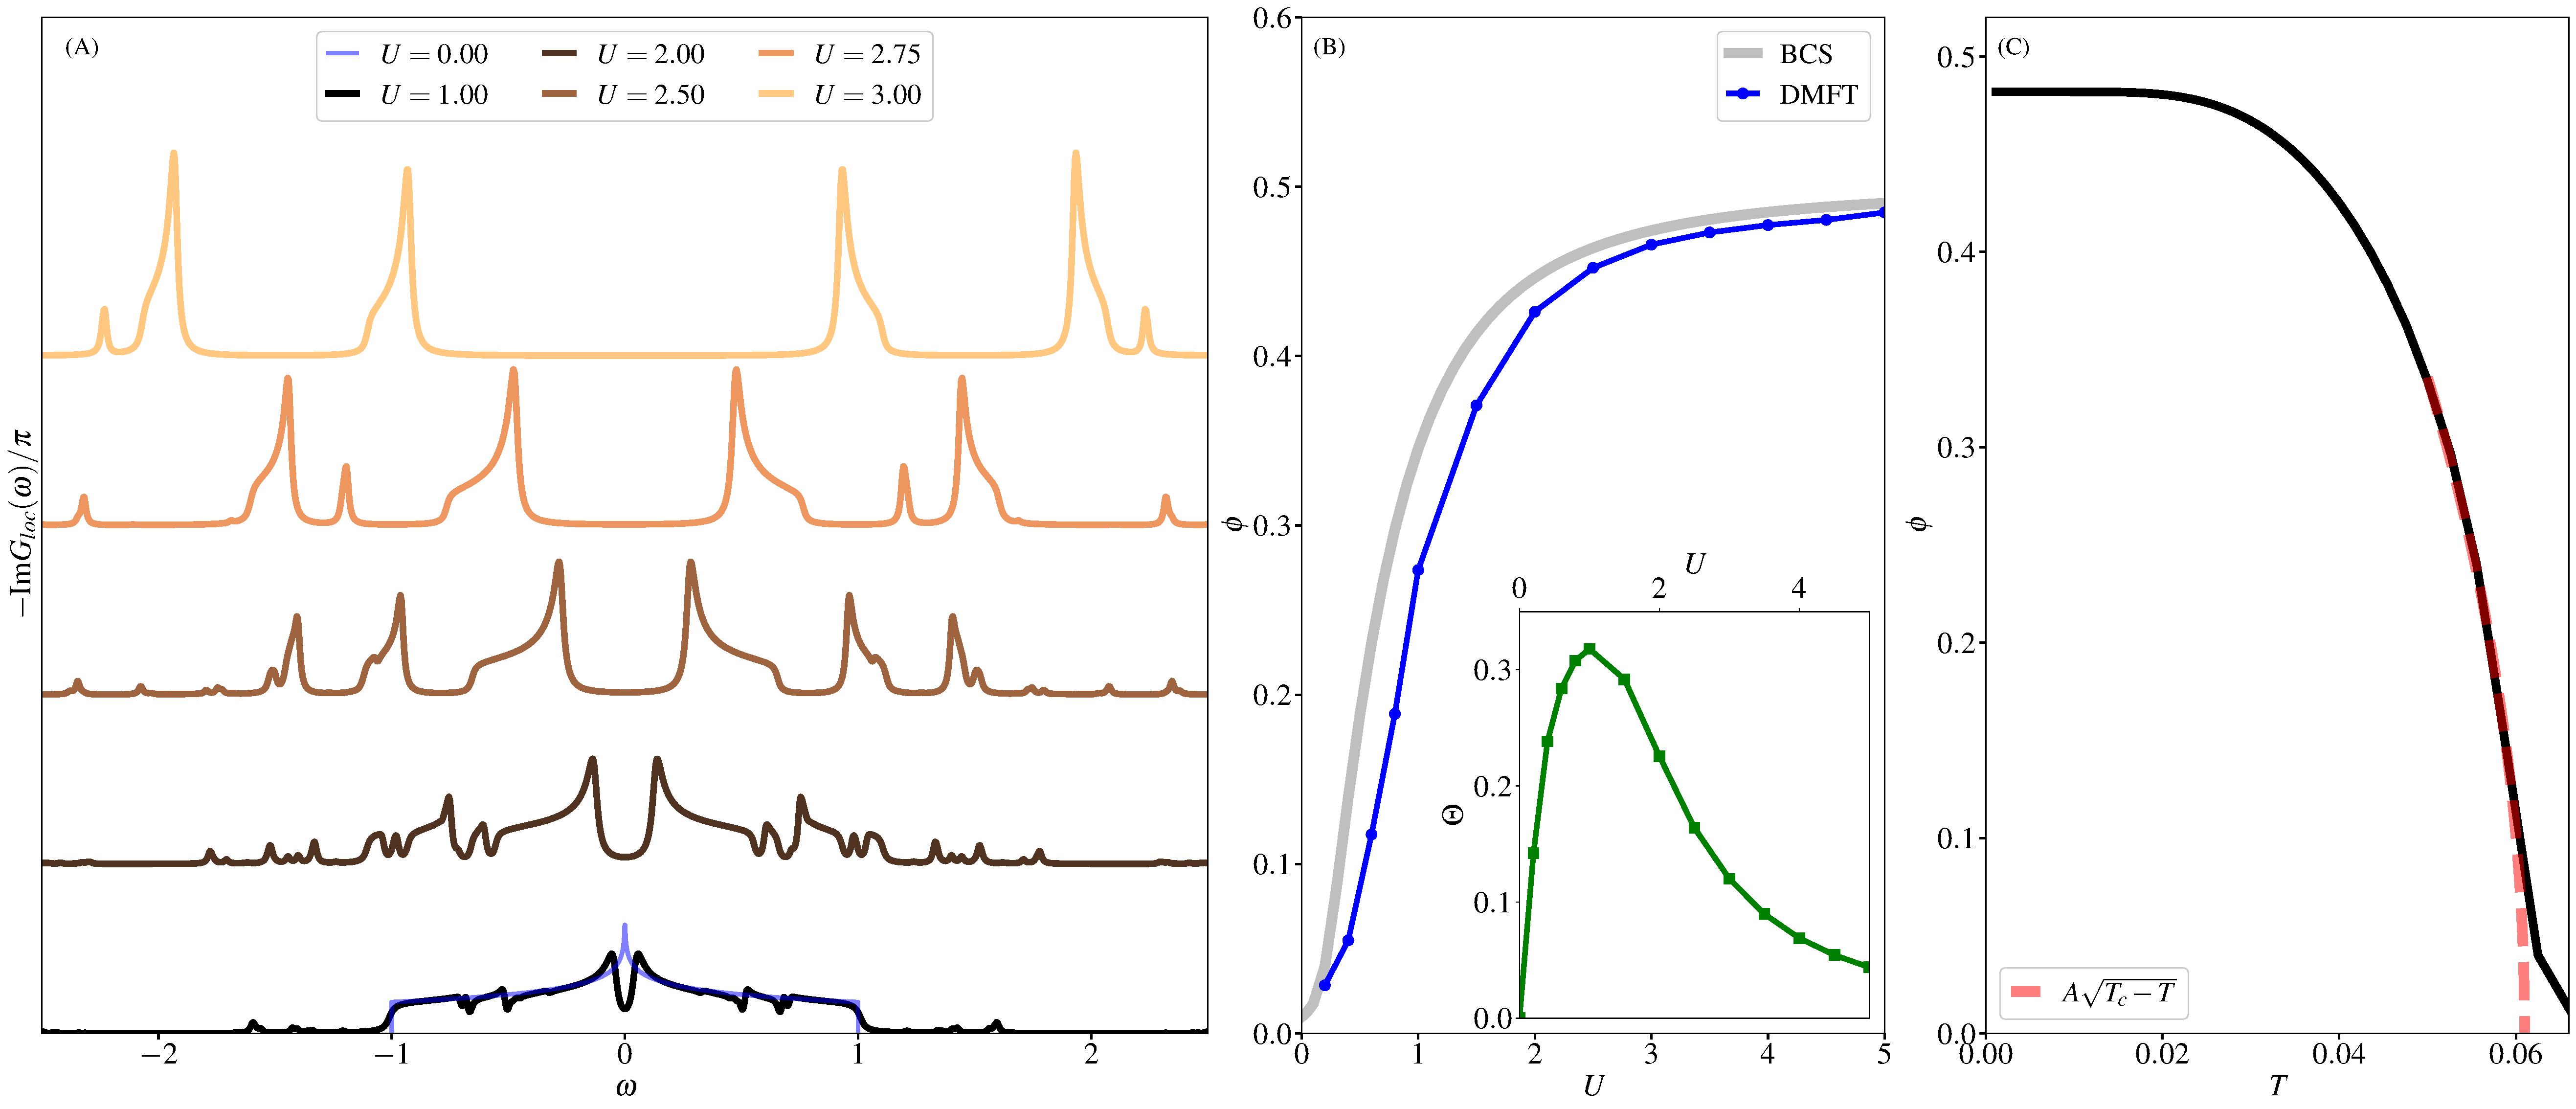
\includegraphics[width=\linewidth]{figures/figAHM.pdf}
    \caption{\label{figEx2}%
      \textbf{The BCS to BEC crossover.}
      (a) Evolution of the spectral functions
      $-\Im{G_\mathrm{loc}(\omega)}/\pi$ as a function of increasing
      attraction $U$. 
      (b) The order parameter $\phi=\langle c_\up c_\dw\rangle$ as a
      function of the attraction $U$. Data for BCS (gray) is compared
      to DMFT results (blue line and symbols). 
      (c) The correlation strength
      $\Theta=\frac{|S(i\omega\to0)-S(i\omega\to\infty)|}{S(i\omega\to\infty)}$ as a function of the
      attraction $U$ across the BCS-BEC crossover. 
      (d) Comparison of the double occupation $D=\langle n_\up
      n_\dw\rangle$ as a function of attraction $U$ between BCS (gray
      solid line) and DMFT (blue solid line and symbols). 
      (e) Superconducting order
      parameter $\phi$ as a function of temperature across the
      superconductor-to-normal phase transition. Data for $U=4$. The
      fit highlights the critical behavior with a mean-field exponent
      $\beta=1/2$ (red dashed line) and parameters $A\simeq 3.7$, $T_\mathrm{c}=0.61$.       
        }
\end{figure}

\paragraph{Results}
Here we showcase some results for the DMFT solution of the 
attractive Hubbard model across the BCS to BEC crossover regime, 
illustrating the capability of \NAME to handle $s$-wave 
superconductivity at both zero and finite temperatures.

To begin, panel (A) of \figu{figEx2} shows the evolution of the 
spectral density, obtained from the local normal Green's function as 
$-\tfrac{1}{\pi}\Im G_\mathrm{loc}(\omega)$, as a function of the 
attraction $U$. For any finite $U$, the Van Hove peak at 
$\omega = 0$ characteristic of the 2D square lattice (visible at 
$U = 0$) is split by the formation of a superconducting gap, whose 
width increases with $U$. This gap reflects the emergence of a finite 
order parameter $\phi = \langle c_\up c_\dw \rangle$, signaling the 
onset of superconducting coherence.


The evolution of this order parameter is presented in panel (B), 
highlighting the crossover from the weak-coupling BCS regime to the 
strong-coupling BEC regime. In the BCS limit, $\phi$ shows the 
characteristic exponential growth with $U$, reflecting the formation 
of weakly bound Cooper pairs. This regime is known to be 
computationally challenging. In the opposite, strong-coupling, limit 
$\phi$ saturates at its theoretical maximum of $\phi \rightarrow 1/2$, 
indicating tightly bound local pairs. Comparison with the mean-field result 
(gray line) reveals the effect of local quantum fluctuations, which 
slightly suppress the order parameter, particularly in the intermediate 
regime.



To quantify these correlation effects, we plot in panel (C) the 
\emph{correlation strength}
$\Theta=\frac{|S(i\omega\to 0)-S(i\omega\to\infty)|}{S(i\omega\to\infty)}$
where $S(i\omega)$ is the anomalous self-energy.
This ratio statically captures 
the maximum amplitude of its dynamical dependence by comparing the high-energy 
mean-field-like limit with the low-energy behavior at the Fermi level. 
Large values of $\Theta$ indicate a strongly correlated state with 
significant dynamical effects, hence a more correlated state.
Our results show that both the weak 
and strong coupling limits are relatively close to the mean-field 
description, while the intermediate regime is marked by strong 
correlations, significantly departing from the BCS picture.

To further illustrate the impact of dynamical correlations, we 
present in panel (D) the evolution of the double occupancy 
$d = \langle n_\up n_\dw \rangle$ as a function of $U$. At half-filling, 
the mean-field expression for this quantity is $d = 1/4 + \phi^2$, 
reflecting the sole contribution of the order parameter. Our DMFT 
results show a slight increase in $d$ over the mean-field prediction 
in the weak coupling regime, indicating enhanced local correlations. 
However, as $U$ increases, the double occupancy quickly drops below 
the mean-field result, reflecting the onset of strong pairing and 
pair localization in the BEC limit.

Finally, we demonstrate the ability of \NAME to capture finite 
temperature effects. Panel (E) shows the temperature dependence of 
the order parameter $\phi(T)$ across the superconducting-to-normal 
transition. The mean-field nature of this transition is evident from 
the scaling near the critical temperature 
$\phi \sim (T_\mathrm{c} - T)^\beta$ with $\beta = 1/2$, consistent 
with classical Ginzburg-Landau theory.

These results collectively illustrate the versatility of \NAME in 
handling both ground state and finite temperature superconducting 
phases, capturing the complex physics of the BCS-BEC crossover with 
high accuracy.


\subsection{Multi-orbital Hubbard (TRIQS)}

\subsection{Some model (W2Dynamics)}

\subsection{Interacting Bernevig-Hughes-Zhang (Fortran)}

\end{document}
